\documentclass[compress]{beamer}

\mode<presentation>
{
  %\usetheme{Warsaw}
  %\usecolortheme{spruce}
  % or ...
	%\useoutertheme{infolines}
  %\setbeamercovered{transparent}
  
  \usetheme{CambridgeUS}
    \setbeamercolor{item projected}{bg=darkred}
    \setbeamertemplate{enumerate items}[default]
    \setbeamertemplate{navigation symbols}{}
    \setbeamercovered{transparent}
    \setbeamercolor{block title}{fg=darkred}
    \setbeamercolor{local structure}{fg=darkred}
  
  % or whatever (possibly just delete it)
}

\usepackage{verbatim} 
\usepackage{listings}
\usepackage{tikz}
\usetikzlibrary{arrows}
\usetikzlibrary{shapes}
\tikzstyle{block}=[draw opacity=0.7,line width=1.4cm]

\newcommand{\bigpause}{\bigskip \pause}

\lstloadlanguages{C++}
\lstnewenvironment{code}
	{%\lstset{	numbers=none, frame=lines, basicstyle=\small\ttfamily, }%
	 \csname lst@SetFirstLabel\endcsname}
	{\csname lst@SaveFirstLabel\endcsname}
\lstset{% general command to set parameter(s)
	language=C++, basicstyle=\footnotesize\sffamily, keywordstyle=\slshape,
	emph=[1]{tipo,usa}, emphstyle={[1]\sffamily\bfseries},
	basewidth={0.47em,0.40em},
	columns=fixed, fontadjust, resetmargins, xrightmargin=5pt, xleftmargin=15pt,
	flexiblecolumns=false, tabsize=2, breaklines,	breakatwhitespace=false, extendedchars=true,
	numbers=left, numberstyle=\tiny, stepnumber=1, numbersep=9pt,
	frame=l, framesep=3pt,
}

\usepackage[spanish]{babel}
% or whatever

\usepackage[utf8]{inputenc}
% or whatever

\usepackage{times}
\usepackage[T1]{fontenc}
% Or whatever. Note that the encoding and the font should match. If T1
% does not look nice, try deleting the line with the fontenc.


\title[Geometr\'ia Computacional] % (optional, use only with long paper titles)
{Geometr\'ia Computacional}

\author[Melanie Sclar] % (optional, use only with lots of authors)
{~Melanie Sclar}
% - Give the names in the same order as the appear in the paper.
% - Use the \inst{?} command only if the authors have different
%   affiliation.
\institute[UBA] % (optional, but mostly needed)
{
  %\inst{1}%
  Facultad de Ciencias Exactas y Naturales\\
  Universidad de Buenos Aires
}
\date[TC 2014] % (optional, should be abbreviation of conference name)
{Training Camp 2014}

% Ac¿ se puede insertar el logo de la UBA
% \pgfdeclareimage[height=0.5cm]{university-logo}{university-logo-filename}
% \logo{\pgfuseimage{university-logo}}



% Delete this, if you do not want the table of contents to pop up at
% the beginning of each subsection:
\AtBeginSubsection[]
{
  \begin{frame}<beamer>{Contenidos}
    \tableofcontents[currentsection,currentsubsection]
  \end{frame}
}

\newcommand{\be}{\begin{equation*}}
\newcommand{\ee}{\end{equation*}}
\newcommand{\state}[1]{\left|\,#1\,\right\rangle}
\newcommand{\costate}[1]{\left\langle\,#1\,\right|}
\newcommand{\trace}{\text{Tr}}
\newcommand{\su}{\uparrow}
\newcommand{\sd}{\downarrow}
\newcommand{\im}{\text{Im}}
\newcommand{\re}{\text{Re}}

% If you wish to uncover everything in a step-wise fashion, uncomment
% the following command:

%\beamerdefaultoverlayspecification{<+->}


\begin{document}
\pgfdeclarelayer{background}
\pgfsetlayers{background,main}
\begin{frame}
  \titlepage
\end{frame}

\begin{frame}{Contenidos}
  \tableofcontents
  % You might wish to add the option [pausesections]
\end{frame}

\section{Introducci\'on}
\begin{frame}

Generalmente, los problemas de geometr\'ia de ACM requieren calcular 
alguna cantidad (por ej., una distancia, un \'area, etc) relacionada con
elementos geom\'etricos como puntos, l\'ineas, c\'irculos, etc.
Para resolverlos, debemos poder ser capaces de:\\
\bigskip
\begin{enumerate}
\item Representar los objetos geom\'etricos involucrados en el problema, 
para poder operar con ellos.

\item Desarrollar un algoritmo para buscar la respuesta deseada.
\end{enumerate}

Entonces, para poder llegar a la segunda parte (la m\'as interesante), primero tenemos que ser capaces de llevar a cabo la primera.

\bigskip

\textbf{Aclaraci\'on:} Nos referiremos siempre a problemas en $\mathbb{R}^2$, ya que son los m\'as comunes.

\end{frame}

\section{Los elementos m\'as b\'asicos: puntos, vectores y rectas}
\begin{frame}[fragile]
Un punto en el plano (o un vector desde el origen hasta dicho punto) se puede representar con un par ordenado de coordenadas en un sistema cartesiano:

\begin{center}
$\vec{P} = (x,y)$ con $x,y \in \mathbb{R}$
\end{center}

\bigskip

Se puede representar como {\tt pair<double,double>}, pero es poco declarativo. Mejor hacer un {\tt struct}:

\begin{lstlisting}
struct Punto {
      double x;
      double y;
};
\end{lstlisting}

\end{frame}

\subsection{Algunas operaciones importantes entre vectores}

\begin{frame}
\begin{itemize}
\item La suma y resta de vectores se realiza componente a componente:
    %
    \be
    \vec{P} = \vec{P}_1 \pm \vec{P}_2  \qquad \Longleftrightarrow \qquad (x, y) = (x_1 \pm x_2, y_1 \pm y_2)
    \ee
    \vspace{0.25cm}
    \item La longitud o \emph{norma} de un vector es $|\vec{P}| = \sqrt{x^2 + y^2}$.
\vspace{0.25cm}
    \item La distancia eucl\'idea entre dos puntos $\vec{P}_1$ y $\vec{P}_2$ es $|\vec{P}_1 - \vec{P}_2|$
\end{itemize}
\end{frame}

\begin{frame}{Producto escalar entre vectores}

\begin{block}{Producto escalar}
El \emph{producto escalar} de dos vectores $u = (x_1,y_1)$ y $v = (x_2,y_2)$ es un n\'umero, y se define como
    %
    \be
    \vec{u} \cdot \vec{v} = x_1 x_2 + y_1 y_2 = |\vec{u}| |\vec{v}| \cos\theta
    \ee
    %
\end{block}
%
    Observar que en particular si $\theta = 90^\circ$ el producto escalar se anula.
\textbf{Es decir, dos vectores son perpendiculares si y s\'olo si su producto escalar da 0}.

\end{frame}

\begin{frame}{Producto cruz entre vectores}

El producto vectorial (o producto cruz) de dos vectores es un \emph{vector} en la direcci\'on normal al plano generado por ellos (¡esto puede ser muy \'util para problemas en $\mathbb{R}^3$!). \\

Si $u,v \in \mathbb{R}^2$ ($u = (x_1,y_1)$ y $v = (x_2,y_2)$), se define $u \times v$ como:
\be
   \vec{u} \times \vec{v} = x_1 y_2 - x_2 y_1
\ee

y se puede demostrar que:

\be
    |\vec{u} \times \vec{v}| = |\vec{u}| |\vec{v}| \sin\theta,
\ee

y que adem\'as \textbf{ $|u \times v|$ es el \'area del paralelogramo determinado por los dos vectores.}

%RELLENAR CON PRODUCTO CRUZ
\end{frame}


\begin{frame}{Producto cruz entre vectores}

El signo del producto indica la orientaci\'on de los vectores.
%
\begin{center}
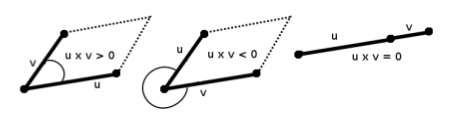
\includegraphics[scale=0.6]{images/producto_cruz.png}
\end{center}
%

Adem\'as, notemos que aqu\'i $u \times v = 0$ significa que los dos vectores tienen igual direcci\'on (¡no confundir con el producto escalar!). \\

\end{frame}

\subsection{Representaci\'on de recta y segmento}
\begin{frame}{¿C\'omo represento una recta?}

Una recta puede ser representada de m\'as de una forma: las dos m\'as usuales son:

\begin{itemize}
\item $L(x) = m x + b$, siendo $m$ la pendiente de la recta y $b$ la ordenada al origen.
\item $L(t) = \mathbf{p} + t \mathbf{v}$, siendo $\mathbf{v} \in \mathbb{R}^2$ el vector direcci\'on y 
$\mathbf{p}$ un punto en la recta. $t \in \mathbb{R}$ es un escalar que representa cu\'anto se dilata o contrae el vector $\mathbf{v}$.
\end{itemize}

El primer enfoque tiene una posible desventaja, ¿cu\'al es?

\bigpause
\invisible<1>{
La pendiente de una recta es un cociente entre dos n\'umeros, y por ende debemos asegurarnos que no se indefina dicho cociente. 
As\'i, si se quiere representar la recta vertical $x = c$, se la deber\'a tratar como un caso especial en el c\'odigo (¡Oh no, un $if$!).
}
\end{frame}

\begin{frame}

Entonces, utilizaremos la representaci\'on $L(t) = p + t v$. ¿C\'omo la obtenemos a partir de dos puntos que pasen por la recta $L$?

\bigpause
\invisible<1>{
Si $a$ y $b$ se encuentran sobre $L$, el vector $v = b-a$ representa la direcci\'on de la recta. Un punto $p$ posible ser\'a el $p = a$. 
As\'i, la recta se escribir\'a como:
\begin{center}
$L(t) = a + t (b-a)$ con $t \in \mathbb{R}$.
\end{center}
}
\end{frame}

\begin{frame}

A partir de esto, podemos representar f\'acilmente un \textbf{segmento de recta} (por ejemplo, la secci\'on de $L$ entre $a$ y $b$). ¿C\'omo?

\bigpause
\invisible<1>{
¡Aprovech\'andonos de $t$! \bigskip

\begin{itemize}
\item Si $t = 0$, $L(0) = a$.
\item Si $t = 1$, $L(1) = b$.
\item Si $0<t<1$, $L(t)$ es parte del segmento determinado por $a$ y $b$.
\item Si $t<0$ o $t>1$, $L(t)$ no ser\'a parte del segmento.
\end{itemize}

Entonces, $L(t)$ pertenece al segmento ya dicho si y s\'olo si $t \in [0,1]$.
}
\end{frame}

%\subsection{Repaso de cuentas importantes}

%producto cruz

%producto escalar

%interseccion linea segmento

%\subsection{Implementaci\'on - buenas pr\'acticas}

\section{Sweep Line (T\'ecnicas de barrido)}

\begin{frame}{¿Qu\'e es sweep line?}
\begin{itemize}
\item La t\'ecnica de \emph{sweep line} se caracteriza por tener una l\'inea (vertical u horizontal generalmente, pero no necesariamente) que va barriendo todo el plano y recolectando informaci\'on sobre puntos de \'el.

\bigskip 
%
\item Si se recuerdan ciertos {\it eventos} que van sucediendo a lo largo del barrido y se los analiza, se pueden obtener soluciones de una complejidad mejor que con otras t\'ecnicas.
\bigskip
\item \textbf{Los eventos ser\'an instantes del barrido en los que sucede algo relevante para el problema.}
\end{itemize}
\end{frame}

\begin{frame}
En alg\'un sentido, la t\'ecnica de sweep line es como la programaci\'on din\'amica: uno aprende la idea general, pero luego en cada problema se aplica y se utiliza de manera diferente, adaptando la idea general ya vista.
\bigskip

Es por eso que creemos que la mejor manera de aprender esta t\'ecnica es viendo algunos ejemplos de problemas relevantes en los que se la utiliza.
\end{frame}

\subsection{Par de puntos m\'as cercano}

\begin{frame}
\begin{block}{Problema}
Dados $n$ puntos en el plano, queremos encontrar dos tales que la distancia entre ellos sea la m\'inima posible (o sea, el par m\'as cercano)
\end{block}
\bigskip
¿Ideas? \pause 
\invisible<1>{
¿C\'omo s\'e qu\'e idea puede funcionar y cu\'al no, si no s\'e cu\'anto vale $n$? Si $n \leq 1000$, el problema a resolver es muy distinto que si $n \leq 1000000$.
}
\end{frame}

\begin{frame}
\begin{itemize}
\item Existe una soluci\'on trivial en $O(n^2)$, que es simplemente mirar cada par y elegir el de menor distancia entre todos los posibles.
\bigskip

\item Es una soluci\'on muy f\'acil de implementar, as\'i que si el problema es con $n \leq 1000$ definitivamente deber\'iamos programar esa.
\bigskip

\item ¿Pero y si $n\leq 1000000$? Utilizaremos sweep line para encontrar una soluci\'on de mejor complejidad.
\end{itemize}
\end{frame}

\begin{frame}
\begin{itemize}
\item El problema con el enfoque $O(n^2)$ es que a cada punto lo comparamos con \textbf{todos} los dem\'as. 
Tal vez podemos aprovecharnos de la posici\'on en el plano de cada uno para no tener que hacer esto cada vez.
\bigskip
\item Barreremos el plano con una recta vertical, de izquierda a derecha.
\bigskip
\item Para ser coherentes con este barrido, ordenaremos los puntos crecientemente seg\'un su coordenada $x$. 
Esto tendr\'a una complejidad de $O(n \lg n)$.
\end{itemize}
\end{frame}


\begin{frame}
\begin{itemize}
\item Llamemos $h$ a la menor distancia entre dos puntos encontrada hasta el momento. 
La inicializaremos en $\infty$ (en la pr\'actica, un valor tan grande tal que sea imposible que haya un par de puntos tan lejanos).

\bigskip

\item Supongamos que ya pasamos por primeros $i-1$ puntos con la l\'inea vertical, y ahora chocamos al $i$-\'esimo punto.
\end{itemize}
\end{frame}

\begin{frame}

Mantendremos un set con los puntos (ya procesados) cuya coordenada $x$ est\'e a una distancia menor a $h$. 
Estos puntos son los \'unicos candidatos a estar a distancia menor que $h$ del punto $i$-\'esimo, y por ende a ser una mejor soluci\'on que la actual. \bigskip

\begin{center}
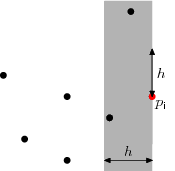
\includegraphics[scale=0.6]{images/closest2.png}
\end{center}
% CAMBIAR EL N POR I EN LA IMAGEN

\end{frame}

\begin{frame}
Tambi\'en fij\'emonos que no cualquier punto cuya coordenada $x$ est\'e a distancia menor a $h$ es un candidato real 
a ser una mejor soluci\'on. Si la coordenada $y$ de un punto est\'a a una distancia mayor a $h$, tampoco ser\'a un candidato. 

\begin{center}
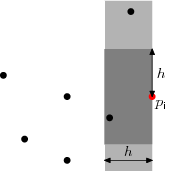
\includegraphics[scale=0.6]{images/closest.png}
\end{center}

\end{frame}

\begin{frame}
As\'i, s\'olo deber\'iamos quedarnos con los puntos cuya coordenada $y$ est\'e en el intervalo $(y_i-h,y_i+h)$. \bigskip

¿C\'omo descartamos los puntos con coordenada $x$ mayor a $h$, si tenemos a los candidatos en un set? \bigpause

\invisible<1>{
¡Manteniendo el set ordenado por su coordenada $y$! 

As\'i, \emph{quitar} los puntos cuya coordenada $y$ est\'a demasiado lejos de $p_i$ se reduce simplemente a no mirar los 
puntos fuera de un intervalo.
%COMO HAGO ESTOOOOO
}
\end{frame}

\begin{frame}

Y ahora, para todos los puntos que quedaron en el set calculamos su distancia con $p_i$ y actualizamos $h$.

¡¿Pero c\'omo?! Potencialmente, hay muchos puntos en el set. \bigpause

\invisible<1>{
Esto no es tan as\'i. Veamos que quedaron a lo sumo 6 candidatos (6 elementos en el set). 
}
\end{frame}

\begin{frame}
La observaci\'on importante es que todos los puntos anteriores est\'an a una distancia mayor o igual a $h$ entre s\'i, 
pues si no, la m\'inima distancia ya habr\'ia sido actualizada anteriormente.

\begin{center}
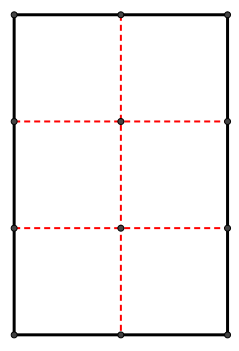
\includegraphics[scale=0.3]{images/seis_cuadrados.png}
\end{center}

No puede haber 2 puntos en el mismo cuadradito, pues luego esos 2 estar\'ian a una distancia menor que $h$. As\'i, hay a 
lo sumo 6 puntos para mirar.

\end{frame}

\begin{frame}{Resumen}

El algoritmo consta de 3 pasos importantes:

\begin{enumerate}
\item Ordenar los puntos por su coordenada x (para poder hacer el barrido con una l\'inea vertical). Esto toma $O(n \lg n)$.
\item Insertar y remover cada punto una vez del set ordenado por coordenada $y$, que toma $O(n \lg n)$ (insertar y remover un elemento toma $O(\lg n)$ usando un set, y hay $n$ puntos en total).
\item Comparar cada punto con una cantidad constante de candidatos ($\leq 6$), lo que toma $O(n)$ en total.
\end{enumerate}
   
As\'i, en total el algoritmo es $O(n \lg n)$!
\end{frame}

\begin{frame}{Problema para pensar}
http://www.spoj.com/problems/CLOSEST/
\end{frame}

\subsection{Intersecci\'on de segmentos}

\begin{frame}
\begin{block}{Problema}
Dados $n$ segmentos en el plano (horizontales o verticales), queremos hallar todas las intersecciones entre dos segmentos.
\end{block}

\bigskip
Nuevamente, si entra en tiempo la soluci\'on trivial $O(n^2)$, hay que programar esa.
\bigskip

Si no, como es por ejemplo el caso $n = 1000000$, tenemos que pensar otra manera de resolverlo. Utilizaremos sweep line.

\end{frame}

\begin{frame}
\begin{itemize}
\item De nuevo utilizaremos un barrido con una l\'inea vertical, pero aqu\'i la situaci\'on es distinta: no ser\'an puntos los que crucen la l\'inea, sino segmentos.
\bigskip
\item Para representarlos, utilizaremos \textbf{eventos}. Los eventos ser\'an coordenadas $x$ en los que pasa algo relevante:
\bigskip
\begin{itemize}
\item Por cada segmento horizontal, habr\'a un evento de apertura (cuando comienza el segmento) y uno de clausura (cuando pasamos por el final del mismo). 
\bigskip

\item Por cada segmento vertical, habr\'a un evento (la aparici\'on del segmento en una cierta coordenada $x$).
\end{itemize}
\end{itemize}
\end{frame}

\begin{frame}[fragile]{Pseudoc\'odigo del algoritmo}

\begin{lstlisting}
lista = la lista de todos los eventos posibles
ordeno lista por las coordenadas x de sus elementos

S = set de segmentos ordenado por la coordenada y de sus elementos
    (inicialmente vacio)

para cada event en lista
    if ( event = horizontal de apertura )
        inserto el segmento en el set S
    if ( event = horizontal de clausura )
        quito el segmento del set S
    if ( event = vertical (segmento de y1 a y2, con y1 < y2) )
        itero los segmentos de S en el rango (y1,y2)
        imprimo las intersecciones halladas

\end{lstlisting}

\textbf{Detalle:} en un set se puede hallar el rango (y1,y2) en $O(\lg n)$,
utilizando las funciones \texttt{lowerbound} y \texttt{upperbound}.

\end{frame}

\begin{frame}{Problema para pensar}
http://goo.gl/UT0O2U (A Safe Bet - WF 2012)
\end{frame}

\subsection{C\'apsula convexa (Convex Hull)}

\begin{frame}
\begin{block}{Problema}
Se tiene un mill\'on vacas en un campo. Se quieren encerrar todas las vacas con una cerca, de manera tal que se minimice la cantidad de alambre utilizado (las vacas deben quedar en el borde o dentro de la cerca).
\end{block}

¿Ideas? \bigpause

\invisible<1>{
Para resolver el problema, tendremos que introducir dos conceptos antes.
}
\end{frame}

\begin{frame}{Pol\'igonos convexos}
\begin{block}{Pol\'igono convexo}
Un pol\'igono es convexo si cumple que dados dos puntos cualesquiera en su interior, el segmento que los une est\'a completamente contenido en \'el.
\end{block}

\begin{center}
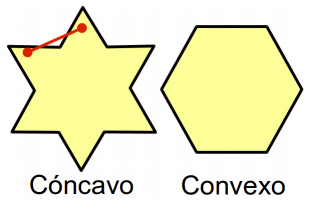
\includegraphics[scale=0.4]{images/convexo.png}
\end{center}

Equivalentemente, un pol\'igono es convexo si los todos sus \'angulos interiores son menores que $180^\circ$.

\bigpause
\invisible<1>{
Notar que el pol\'igono que ser\'a soluci\'on al problema debe ser convexo.
}
\end{frame}


\begin{frame}
\begin{block}{C\'apsula convexa}
Dados $n$ puntos, la \emph{c\'apsula convexa} es el menor pol\'igono convexo que contiene a todos los puntos 
en su interior. Se puede probar que es \'unica.
\end{block}

\begin{center}
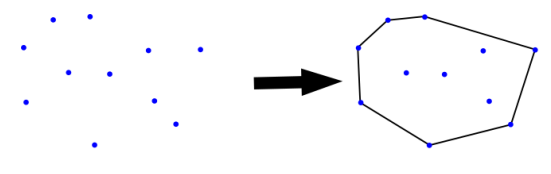
\includegraphics[scale=0.5]{images/convex_hull.png}
\end{center}

\invisible<1>{
\pause 
Entonces, podemos ver que el problema se reduce a hallar la c\'apsula convexa. ¿Pero c\'omo lo hacemos?
}
\end{frame}

\begin{frame}{Algoritmo de Graham Scan}

Se elige el punto de m\'as abajo (con menor $y$), y en caso de haber m\'as de un punto con la misma $y$ se elige el punto de m\'as a la izquierda (o sea, con menor $x$). A este punto lo llamaremos $P$. Elegirlo tiene una complejidad $O(n)$.

\bigskip

\begin{center}
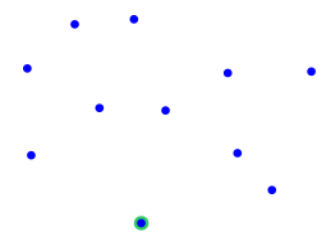
\includegraphics[scale=0.5]{images/convex_hull1.png}
\end{center}

\end{frame}

\begin{frame}
\textbf{Iremos barriendo el plano con una semirrecta que parta desde $P$}. Esta semirrecta no ser\'a vertical ni horizontal, como ven\'iamos viendo, sino que \textbf{girar\'a en sentido antihorario}.

\bigpause
\invisible<1>{
Para poder hacerlo, tenemos que ordenar los puntos por su \'angulo respecto a $P$ y al eje $x$. Si dos puntos tienen el mismo \'angulo, desempatamos por el m\'as cercano primero.

\begin{center}
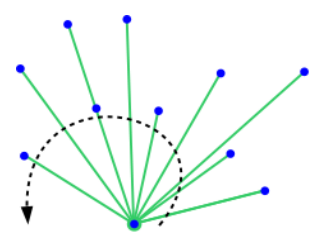
\includegraphics[scale=0.5]{images/convex_hull2.png}
\end{center}
}
\end{frame}

\begin{frame}
Ahora veamos c\'omo manejamos los eventos (en este caso, ser\'a simplemente la aparici\'on de un punto en el barrido).\bigskip

El pr\'oximo punto siempre est\'a en la Convex Hull. En este caso, $u\times v > 0$.

\begin{center}
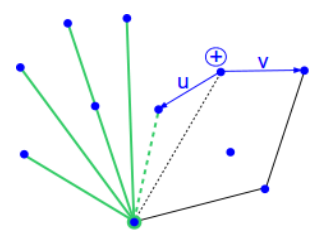
\includegraphics[scale=0.5]{images/convex_hull3.png}
\end{center}

\end{frame}

\begin{frame}
Mientras que $u\times v < 0$, sacamos el punto anterior (¡forma un \'angulo mayor que $180^\circ$!).

\begin{center}
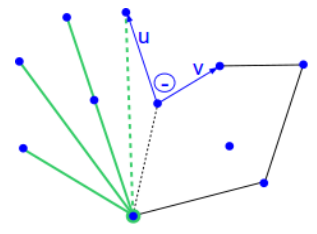
\includegraphics[scale=0.5]{images/convex_hull4.png}
\end{center}

\end{frame}

\begin{frame}[fragile]{Pseudoc\'odigo del Graham Scan}

\begin{lstlisting}
vector<Punto> ConvexHull ( vector<Punto>& lista ) {
    if( |lista| < 3 ) devolver lista
    p = el punto de mas abajo y mas a la izquierda
    Ordenar todos los puntos por angulo respecto a p
        (desempatando por distancia a p, los mas cercanos primero)
    pila = stack de puntos vacio
    pila.push(lista[0]) // lista[0] == p
    pila.push(lista[1])
    i = 2
    while (i < N)
        sea a el tope de pila, b el anteultimo de la pila (si existen)
        if (pila.size > 1 && pcruz(lista[i] - a , b - a) <= 0 )
            pila.pop()
        else
            pila.push(lista[i])
            i = i + 1
    devolver pila
}
\end{lstlisting}

\end{frame}

\begin{frame}{Problemas para pensar}

\begin{itemize}
\item goo.gl/rT7Ji
\item goo.gl/llEHC
\end{itemize}

\end{frame}

\section{\'Area de un pol\'igono}

\begin{frame}{\'Area de un tri\'angulo}
¿Y si adem\'as de pedirnos el pol\'igono que minimiza la cantidad de alambre necesario para encerrar todas las vacas nos hubieran pedido la superficie que tiene dicho pol\'igono?

\bigpause
\invisible<1>{
Comencemos de lo m\'as sencillo: primero pensemos c\'omo sacar\'iamos el \'area de un tri\'angulo.
} 
\bigpause

\invisible<1-2>{
Recordemos lo que vimos hace un rato: si $u$ y $v$ son dos vectores que forman un \'angulo $\theta$, $|u \times v|$ es igual al \'area del paralelogramo que forman.

\begin{center}
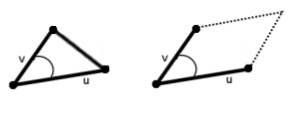
\includegraphics[scale=0.6]{images/producto_cruz_triangulo.png}
\end{center}
}
\end{frame}

\begin{frame}

As\'i, el \'area del tri\'angulo marcado es $\displaystyle\frac{|u\times v|}{2}$.\bigpause

\invisible<1>{
¿C\'omo podemos aplicar lo ya visto para sacar el \'area de un pol\'igono? 
}

\bigpause

\invisible<1-2>{
¡Triangulando! Ve\'amoslo.
}
\end{frame}

\begin{frame}

Se triangula desde un v\'ertice cualquiera y se suman \textbf{en orden} los productos cruz. La superficie del pol\'igono es la mitad del valor absoluto de este n\'umero.

\begin{center}
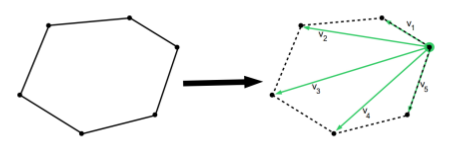
\includegraphics[scale=0.6]{images/triangulacion.png}
\end{center}

Si el pol\'igono es c\'oncavo, sigue valiendo el mismo algoritmo.
\bigpause

Complejidad: $O(n)$ si $n$ es la cantidad de v\'ertices del pol\'igono.

\end{frame}

\begin{frame}{Teorema de Pick}

{\footnotesize
\begin{itemize}
\item $A$ es el \'area del pol\'igono.
\item $I$ es la cantidad de puntos interiores.
\item $B$ es la cantidad de puntos del borde. Se pueden calcular usando
el MCD de la longitud en $x$ y en $y$ de cada lado.
\end{itemize}

$$ A = I + \displaystyle \frac{B}{2} -1 $$}

\begin{center}
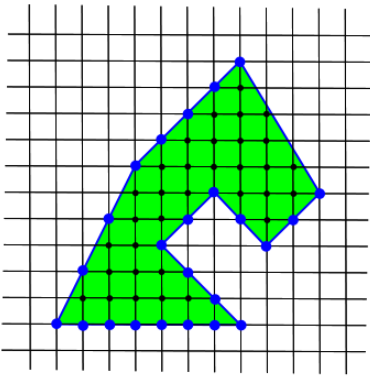
\includegraphics[scale=0.3]{images/pick.png}
\end{center}

\end{frame}

\begin{frame}{Referencias}
   \begin{itemize}
   \item \textit{Introduction to Algorithms, 2nd Edition}. MIT Press. \\ Thomas H. Cormen
   \textbf{Sección 33} (Computational Geometry)
   \item \url{https://www.topcoder.com/tc?module=Static&d1=tutorials&d2=geometry1}
   \item \url{https://www.topcoder.com/tc?module=Static&d1=tutorials&d2=geometry2}
   \item \url{https://www.topcoder.com/tc?module=Static&d1=tutorials&d2=geometry3}
   \item \url{https://www.topcoder.com/tc?module=Static&d1=tutorials&d2=lineSweep}
  \end{itemize}
  
\end{frame}


\end{document}
